\chapter{Catalogazione delle vulnerabilità}
Per vulnerabilità del software si intende una
debolezza presente, comprensibile e sfruttabile
da un attaccante. Vediamo il ciclo di vita di una vulnerabilità:
\begin{enumerate}
    \item Rilascio di un software da un venditore
    \item Scoperta della vulnerabilità da parte di un attaccante
e rilascio di un exploit
    \item Scoperta della vulnerabilità da parte del venditore
    \item Divulgazione della vulnerabilità al pubblico
    \item Rilevazione dell’exploit da parte degli anti-virus
    \item Rilascio di una patch da parte del venditore
    \item Mitigazione dell’exploit su tutti i sistemi 
\end{enumerate}

\begin{figure}[hbpt!]
    \centering
    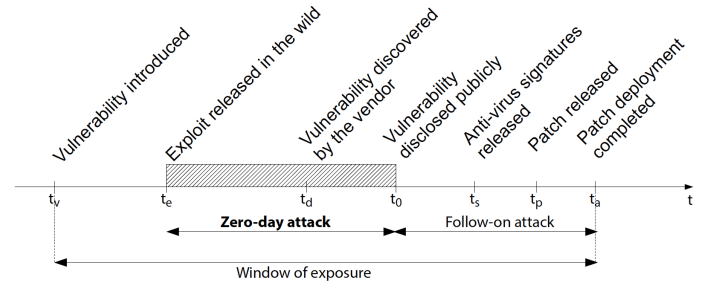
\includegraphics[width=0.7\textwidth]{./Images/cap2/2.1.png}
\end{figure}
\FloatBarrier

L'attacco effettuato nel periodo \([t_e, t_0]\) viene detto \textbf{zero-day attack}, mentre quello effettuato nel periodo \([t_0, t_a]\) avviene in presenza della conoscenza pubblica della vulnerabilità. Più vicini si è allo zero-day, più è probabile che un attacco al software abbia successo.

\vspace{5mm}

Spesso vengono dati delle ricompense in denaro per chi riesce a sfruttare vulnerabilità zero-day: è il caso di Zerodium, azienda di sicurezza informatica fondata nel 2015 che offre ricompense fino a due milioni e mezzo di dollari a chi fornisce zero-day exploit. Nel 2015 Zerodium è arrivata ad offrire un milione di
dollari per attacchi zero-day contro iOS 9. A Maggio 2020 Zerodium ha annunciato con un tweet
di non essere più interessata ad exploit contro iOS. Le prime avvisaglie di questo cambio di rotta si erano
già avute con l’aggiornamento dei “listini” che
mostravano maggior interesse per Android. Nel 2021 Zerodium ha mostrato interesse verso
exploit per i servizi di VPN di Windows. In particolare, interessano exploit che portino a
\begin{itemize}
    \item esposizione di informazioni confidenziali
    \item violazione dell’anonimato
    \item esecuzione di codice arbitrario
\end{itemize}
È importante tenere traccia delle vulnerabilità note, e ciò può essere fatto mediante enumerazione, ovvero costruzione di una tupla univoca per ciascuna vulnerabilità: (id, tipo vulnerabilità, vettore di attacco, minaccia, exploit), oppure per catalogazione: inserimento della tupla in un archivio. Sono stati proposti diversi archivi indipendenti, con relativi problemi di duplicazione e eterogeneità.

\section{Common Vulnerability Exposure}
Nel 1999 il MITRE, un ente no-profit, ha introdotto un
catalogo uniforme delle vulnerabilità: il Common Vulnerability Exposures (CVE)
disponibile al link https://cve.mitre.org.

Le vulnerabilità presenti nel CVE violano almeno una proprietà nella triade CIA (Confidentiality, Integrity, Availability), e sono identificate da una stringa univoca CVE-ANNO-NUMERO. Inoltre sono descritte da una scheda esplicativa contenente descrizione, URL a una pagina dettagliata (References) e data di creazione.

\vspace{5mm}

\subsubsection{Esempio: CVE-2014-0160}
Si tratta di una vulnerabilità della libreria
crittografica Open SSL, resa nota al
pubblico nell’Aprile 2014. OpenSSL, fin dal 1998, è largamente utilizzata nelle
applicazioni Web per la protezione delle informazioni
scambiate tra client e server. Tale vulnerabilità, detta “Heartbleed”
,
consentiva di violare la confidenzialità delle
informazioni protette mediante il protocollo SSL/TLS. Oltre il 60\% dei server Web era vulnerabile all’attacco. Successivamente fu rilasciata una nuova versione di
OpenSSL che eliminava il difetto.

\begin{figure}[hbpt!]
    \centering
    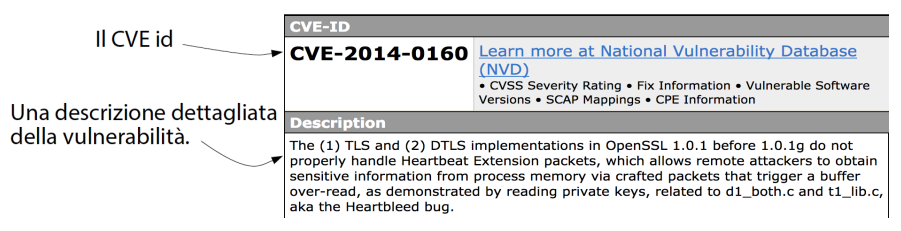
\includegraphics[width=0.9\textwidth]{./Images/cap2/2.2.png}
\end{figure}
\FloatBarrier

\begin{figure}[hbpt!]
    \centering
    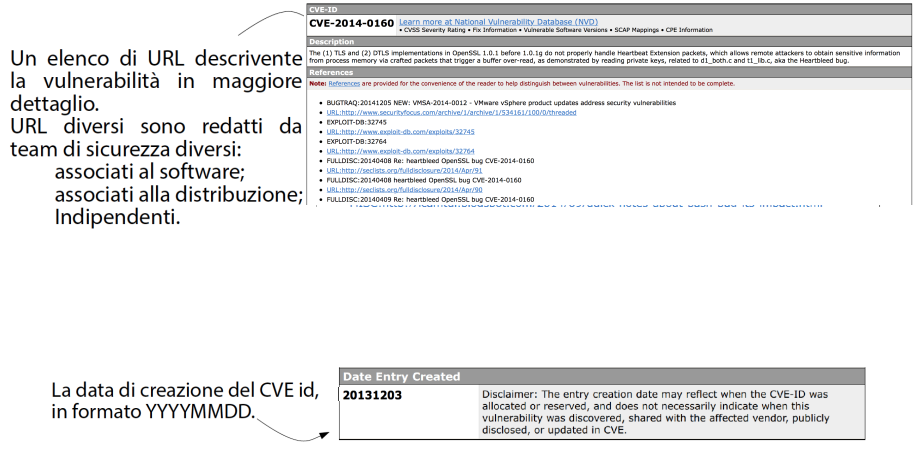
\includegraphics[width=0.9\textwidth]{./Images/cap2/2.3.png}
\end{figure}
\FloatBarrier
Heartbleed è causata da una impropria validazione degli
input all’interno dell’implementazione della estensione
heartbeat di TLS. Usando tale estensione, ciascuna delle due parti comunicanti
conferma all’altra la propria presenza inviando un pacchetto
(heartbeat payload) contenente alcuni dati testuali. L’attacco consiste nell’inviare informazioni false relative alla
lunghezza del payload. Dichiarando che la lunghezza del payload è la massima possibile
(64KB), il server che riceve il pacchetto risponde copiando la
quantità di memoria richiesta. Tale memoria può contenere qualsiasi cosa (chiavi di cifratura,
password, etc.)
Heartbleed è un esempio di mancata validazione degli input.

\subsubsection{Esempio: CVE-2014-6271}
Si tratta di una vulnerabilità della shell BASH,
resa nota al pubblico nel Settembre 2014. BASH, proposta nel 1989 in sostituzione della Bourne shell,
è la shell di default per molte distribuzioni Linux e MacOS. Tale vulnerabilità, detta “Shellshock”, consentiva
l’esecuzione di codice arbitrario anche da remoto! Nel giro di pochi giorni furono portati a termine milioni di
attacchi, principalmente di tipo DDoS. Successivamente fu rilasciata una nuova
versione della shell BASH che eliminava
il difetto.

\begin{figure}[hbpt!]
    \centering
    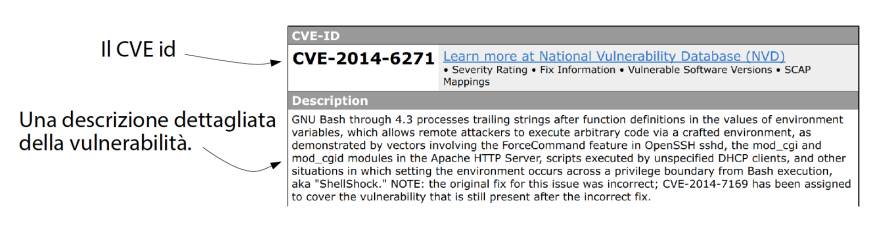
\includegraphics[width=0.9\textwidth]{./Images/cap2/2.4.png}
\end{figure}
\FloatBarrier

\begin{figure}[hbpt!]
    \centering
    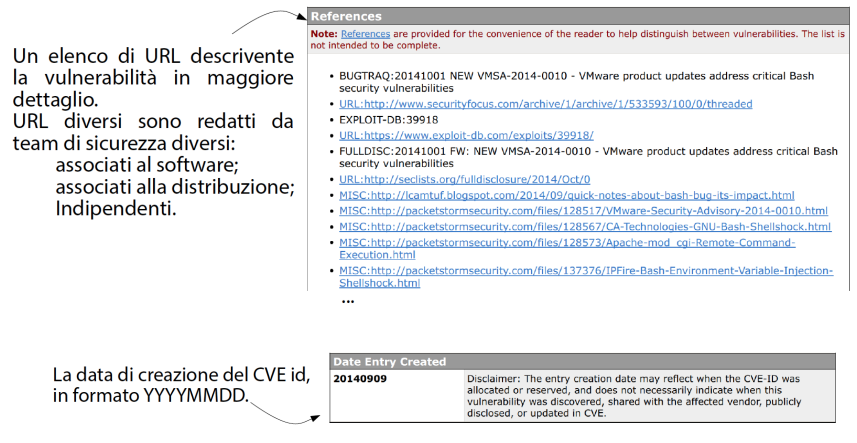
\includegraphics[width=0.9\textwidth]{./Images/cap2/2.5.png}
\end{figure}
\FloatBarrier

BASH consente di esportare variabili e funzioni di
ambiente, rendendole disponibili alle shell figlie:

\vspace{5mm}

\texttt{\$ export foo=' () \{ echo "In foo";\}'}

\texttt{\$ bash -c 'foo'}

\texttt{In foo}

\vspace{5mm}

Supponiamo di concatenare un altro comando al
termine della definizione della funzione foo:

\vspace{5mm}

\texttt{\$ export foo=' () \{ echo "In foo";\};}

\texttt{echo vulnerable'}

\vspace{5mm}

Cosa accade se viene invocata una shell figlia?

\vspace{5mm}

\texttt{\$ bash -c 'foo'}

\vspace{5mm}

Viene visualizzato:

\vspace{5mm}

\texttt{vulnerable}

\texttt{In foo}

\vspace{5mm}

Se l’attaccante ha accesso al file di inizializzazione \texttt{.bashrc}
può inserire la seguente definizione di funzione di ambiente:

\vspace{5mm}

\texttt{\$ export foo=' () \{ echo "In foo";\}; evil\_command'}

\vspace{5mm}

Ogni volta che l’utente vittima apre una shell BASH viene
eseguito il comando \texttt{evil\_command}. Questo attacco è un esempio di escalation of privilege.

Ma il problema è ben più serio perché l’attacco è
eseguibile anche da remoto.
Ogni server remoto che accetta codice BASH e lo valuta
senza controllarlo è potenzialmente attaccabile. Ad esempio, quando il Web server Apache esegue uno script
scritto in BASH, salva gli header della richiesta in variabili di
ambiente e le valuta. È sufficiente costruire una linea BASH maligna e passarla
come header di una richiesta (maliziosa) per sfruttare la
vulnerabilità da remoto. Possiamo utilizzare il comando curl per iniettare un
header malformato in modo da provocare l’esecuzione
di \texttt{evil\_command}.

\vspace{5mm}

\texttt{\$ curl -v http://server/cgi-bin/bashcgi -H}

\texttt{"custom:() \{ :; \} ; evil\_command"}

\vspace{5mm}

In questo modo viene invocato lo script \texttt{bashcgi}
Ø Viene passato un header HTTP di nome “custom” col
valore sopra specificato
Ø In accordo a RFC3875, Apache crea una variabile di
ambiente \texttt{HTTP\_CUSTOM} per lo script \texttt{bashcgi}. A questo punto Lo script \texttt{bashcgi} viene eseguito e la variabile di
ambiente viene valutata. Il comando \texttt{evil\_command} è eseguito sul server con i
diritti dell’utente con sui esegue Apache! 

\subsubsection{Shellshock VS Heartbleed}
Shellshock è una vulnerabilità molto più
seria di Heartbleed: mentre Heartbleed consente agli
attaccanti di rubare dati confidenziali, Shellshock consente di eseguire codice
arbitrario da remoto. Infatti il livello di severità di Shellshock è 10, mentre quello di Heartbleed è 5.

\section{Common Vulnerability Scoring System}
IL CVE enumera le vulnerabilità, ma non ne misura
l’impatto. Non stabilisce quale tra le vulnerabilità debba essere
gestita più urgentemente. Non stabilisce come le vulnerabilità possano impattare
su sistemi diversi. Per questo motivo è stato introdotto il
Common Vulnerability Scoring System (CVSS), che stima la gravità di ogni vulnerabilità: assegna ad ogni CVE id un punteggio da 0 a 10:
\begin{itemize}
    \item 0: impatto nullo
    \item (0,4): impatto basso
    \item (4,7): impatto medio
    \item (7,9): impatto elevato
    \item (9,10): impatto critico 
\end{itemize}
Due versioni del CVSS sono correntemente in uso
\begin{itemize}
    \item Versione 2 (v2): introdotta nel 2005, pubblicata nel 2007
    
https://www.first.org/cvss/v2/guide
    \item Versione 3 (v3): introdotta nel 2012, pubblicata nel 2015
    
    https://www.first.org/cvss/specification-document
\end{itemize}
Entrambe assegnano il punteggio in base a tre gruppi
di metriche:
\begin{itemize}
    \item Base (Base Metric): stimano la gravità della vulnerabilità, a prescindere da
fattori temporali e ambientali. Rispondono alle domande:
\begin{itemize}
    \item Qual è il vettore di attacco?
    \item Quanto è semplice sfruttare la vulnerabilità?
    \item Qual è l’impatto sulla triade delle proprietà CIA?
\end{itemize}
    \item Temporali (Temporal Metric): stimano la gravità della vulnerabilità dal punto di vista
temporale. Rispondono alle domande:
\begin{itemize}
    \item E’ disponibile un exploit?
    \item E’ disponibile una patch?
\end{itemize}
    \item Ambientali (Environmental Metric): stimano la gravità della vulnerabilità dal punto di vista
ambientale. Rispondono alle domande:
\begin{itemize}
    \item Qual è la conseguenza di un exploit su persone e cose?
    \item Quanti sistemi sono vulnerabili? 
\end{itemize}
\end{itemize}
\begin{figure}[hbpt!]
    \centering
    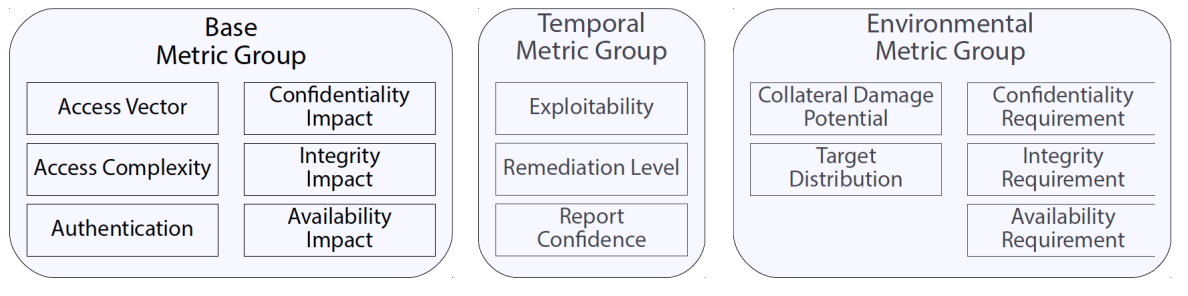
\includegraphics[width=0.9\textwidth]{./Images/cap2/2.7.png}
\end{figure}
\FloatBarrier
Ad ogni metrica è associata una domanda
a risposta multipla, e ciascuna risposta fornisce un peso numerico. I singoli pesi sono poi aggregati in un
risultato finale tramite una serie di formule. Entriamo nei dettagli di ciascuna metrica
e vediamo come sono associati i punteggi.
\subsection{Metriche Base}
\subsubsection{Access Vector}
Tramite quale vettore di accesso può essere
sfruttata la vulnerabilità? Alla metrica AV (Access Vector) può essere assegnato uno
dei tre valori L (Local), A (Adjacent Network), N (Network).

\begin{figure}[hbpt!]
    \centering
    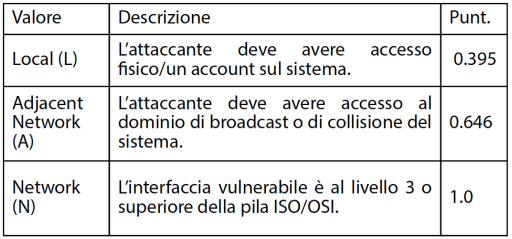
\includegraphics[width=0.4\textwidth]{./Images/cap2/2.8.png}
\end{figure}
\FloatBarrier

\subsubsection{Access Complexity}
Quanto è difficile sfruttare la vulnerabilità? Alla metrica AC (Access Complexity) può essere assegnato uno
dei tre valori H (High), M (Medium), L (Low). 

\begin{figure}[hbpt!]
    \centering
    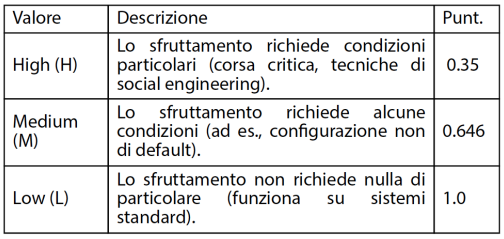
\includegraphics[width=0.4\textwidth]{./Images/cap2/2.9.png}
\end{figure}
\FloatBarrier

\subsubsection{Authentication}
Quante volte un attaccante si deve
autenticare per sfruttare la vulnerabilità? Alla metrica A (Authentication) può essere assegnato uno
dei tre valori M (Multiple), S (Single), N (None).

\begin{figure}[hbpt!]
    \centering
    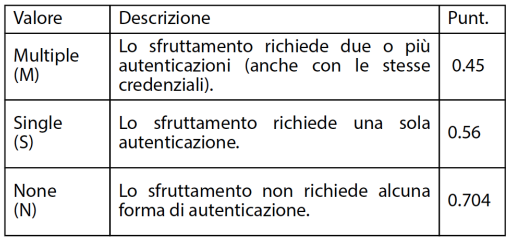
\includegraphics[width=0.4\textwidth]{./Images/cap2/2.10.png}
\end{figure}
\FloatBarrier

\subsubsection{Confidentiality Impact}
Qual è l’impatto della vulnerabilità
sulla confidenzialità del sistema? Alla metrica CI (Confidentiality Impact) può essere assegnato uno
dei tre valori N (None), P (Partial), C (Complete).

\begin{figure}[hbpt!]
    \centering
    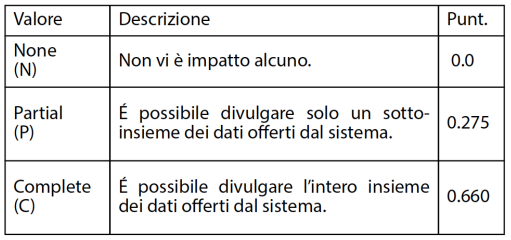
\includegraphics[width=0.4\textwidth]{./Images/cap2/2.11.png}
\end{figure}
\FloatBarrier

\subsubsection{Integrity Impact}
Qual è l’impatto della vulnerabilità
sull’integrità del sistema? Alla metrica II (Integrity Impact) può essere assegnato uno
dei tre valori N (None), P (Partial), C (Complete).

\begin{figure}[hbpt!]
    \centering
    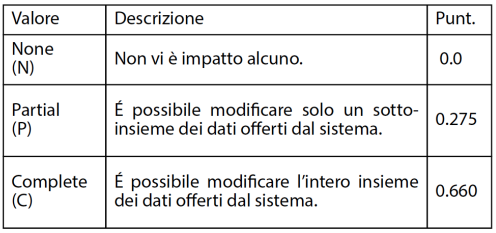
\includegraphics[width=0.4\textwidth]{./Images/cap2/2.12.png}
\end{figure}
\FloatBarrier

\subsubsection{Availability Impact}
Qual è l’impatto della vulnerabilità
sulla disponibilità del sistema? Alla metrica AI (Availability Impact) può essere assegnato uno
dei tre valori N (None), P (Partial), C (Complete).

\begin{figure}[hbpt!]
    \centering
    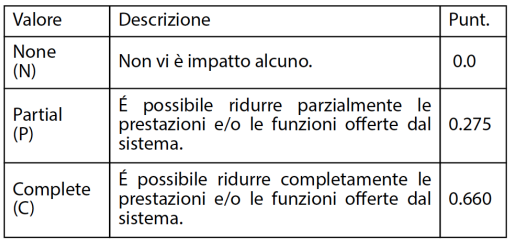
\includegraphics[width=0.4\textwidth]{./Images/cap2/2.13.png}
\end{figure}
\FloatBarrier

\subsubsection{Calcolo del punteggio}
Le risposte relative alle metriche base sono
presentate sotto forma di stringa di testo. Tale stringa, detta \textit{vector string}, è formata da coppie
di abbreviazioni metrica:risposta separate dal
carattere slash. Esempio: 
\vspace{5mm}
\begin{center}
AV:N/AC:L/Au:N/C:P/I:P/A:C  
\end{center}
\vspace{5mm}
Il Punteggio Base stima la gravità della vulnerabilità
senza considerare fattori temporali ed ambientali.


\[Exploitability = 20 \times AccessVector \times AccessComplexity \times Authentication\]
\[Impact = 10.41 \times (1-(1- ConflImpact)\times(1-IntegImpact)\times(1-AvailImpact))\]

\[f(Impact) = \begin{dcases*}
        0 & if $Impact = 0$\\
        1.176 & otherwise. 
        \end{dcases*}
        \]
\[BaseScore = roundTo1Decimal(((0.6 \times Impact)+(0.4 \times Exploitability)-1.5) \times f(Impact)\]

I punteggi associati alle altre due metriche sono
opzionali: si calcolano nello stesso modo (con questionari diversi) le relazioni tra i punteggi, e il Punteggio Temporale ingloba il Punteggio Base, mentre il Punteggio Ambientale ingloba il Punteggio Temporale.

\begin{figure}[hbpt!]
    \centering
    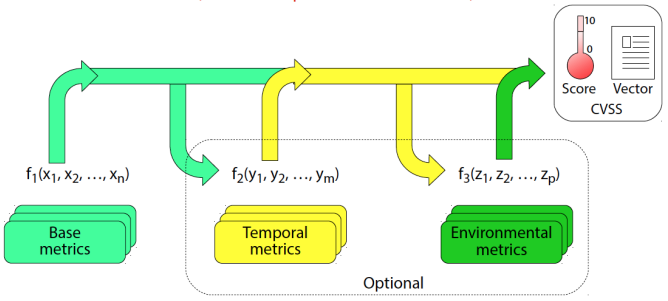
\includegraphics[width=0.6\textwidth]{./Images/cap2/2.14.png}
\end{figure}
\FloatBarrier

\subsection{Metriche Temporali}
\subsubsection{Exploitability}
Qual è lo stato attuale delle tecniche
di sfruttamento della vulnerabilità? Alla metrica E (Exploitability) può essere assegnato uno
dei cinque valori U (Unproven), P (Proof of Concept),
F (Functional), H (High), ND (Not Defined).

\begin{figure}[hbpt!]
    \centering
    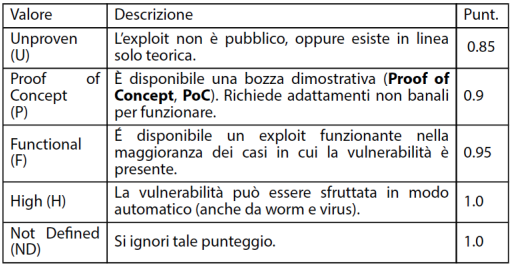
\includegraphics[width=0.4\textwidth]{./Images/cap2/2.15.png}
\end{figure}
\FloatBarrier

\subsubsection{Remediation Level}
E’ presente un rimedio per
mitigare la vulnerabilità? Alla metrica RL (Remediation Level) può essere assegnato uno
dei cinque valori O (Official fix), T (Temporary fix),
W (Workaround), U (Unaivalable), ND (Not Defined).

\begin{figure}[hbpt!]
    \centering
    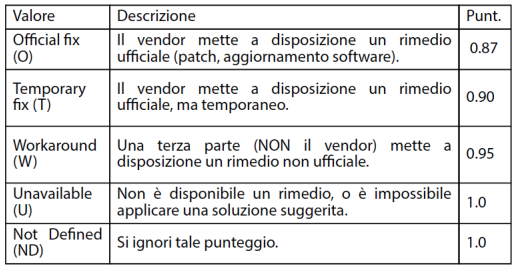
\includegraphics[width=0.4\textwidth]{./Images/cap2/2.16.png}
\end{figure}
\FloatBarrier

\subsubsection{Report Confidence}
La vulnerabilità esiste veramente?
E’ descritta in maniera credibile? Alla metrica RC (Report Confidence) può essere assegnato uno
dei quattro valori UC (Unconfirmed), UR (Uncorroborated),
C (Confirmed), ND (Not Defined).

\begin{figure}[hbpt!]
    \centering
    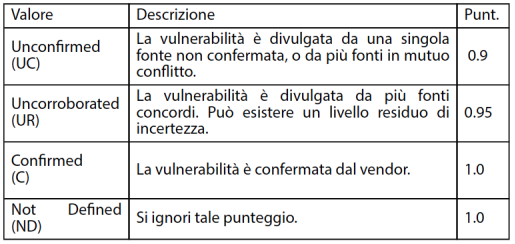
\includegraphics[width=0.4\textwidth]{./Images/cap2/2.17.png}
\end{figure}
\FloatBarrier

\subsubsection{Calcolo del Punteggio Temporale}
Il Punteggio Temporale stima la gravità della
vulnerabilità includendo il fattore temporale:

\[TemporalScore = roundTo1Decimal(BaseScore \times Exploitab \times RemedLvl \times ReportConf)\]

\subsection{Metriche Ambientali}
\subsubsection{Collateral Damage Potential}
Qual è l’impatto della vulnerabilità sui sistemi fisici,
sulle persone e sulle risorse finanziarie? Alla metrica CDP (Collateral Damage Potential) può essere assegnato
uno dei sei valori N (None), L (Low), LM (Low-Medium),
MH (Medium-High), H (High), ND (Not Defined).

\begin{figure}[hbpt!]
    \centering
    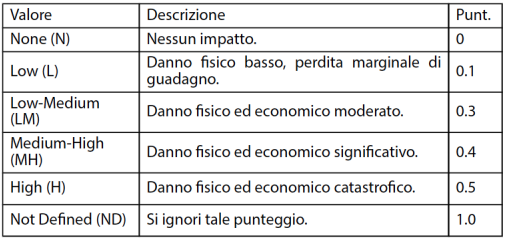
\includegraphics[width=0.4\textwidth]{./Images/cap2/2.18.png}
\end{figure}
\FloatBarrier

\subsubsection{Target Distribution}
Quale percentuale di asset
è soggetta alla vulnerabilità? Alla metrica TD (Target Distribution) può essere assegnato uno
dei cinque valori N (None), L (Low),
M (Medium), H (High), ND (Not Defined).

\begin{figure}[hbpt!]
    \centering
    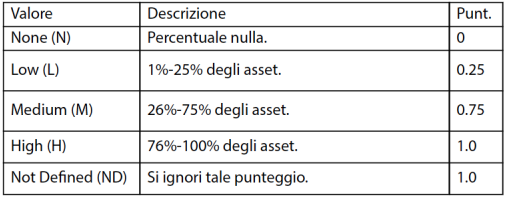
\includegraphics[width=0.4\textwidth]{./Images/cap2/2.19.png}
\end{figure}
\FloatBarrier

\subsubsection{Confidentiality Requirement}
Qual è l’impatto di una
perdita di confidenzialità? Alla metrica CR (Confidentiality Requirement) può essere
assegnato uno dei quattro valori
L (Low), M (Medium), H (High), ND (Not Defined).

\begin{figure}[hbpt!]
    \centering
    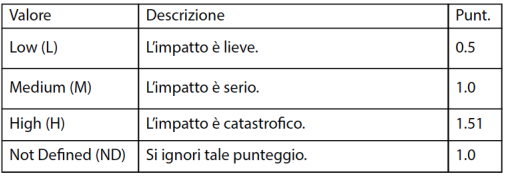
\includegraphics[width=0.4\textwidth]{./Images/cap2/2.20.png}
\end{figure}
\FloatBarrier

\subsubsection{Integrity Requirement}
Qual è l’impatto di una
perdita di integrità? Alla metrica IR (Integrity Requirement) può essere assegnato
uno dei quattro valori
L (Low), M (Medium), H (High), ND (Not Defined).

\begin{figure}[hbpt!]
    \centering
    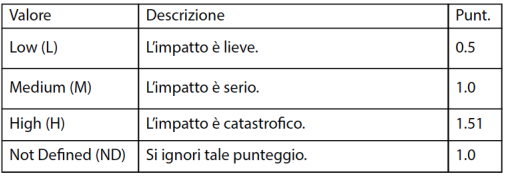
\includegraphics[width=0.4\textwidth]{./Images/cap2/2.20.png}
\end{figure}
\FloatBarrier

\subsubsection{Availability Requirement}
Qual è l’impatto di una
perdita di disponibilità? Alla metrica AR (Availability Requirement) può essere assegnato
uno dei quattro valori
L (Low), M (Medium), H (High), ND (Not Defined).

\begin{figure}[hbpt!]
    \centering
    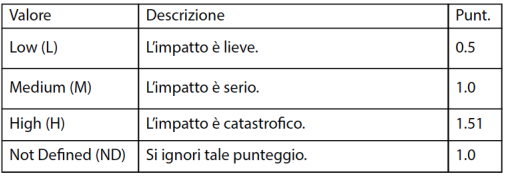
\includegraphics[width=0.4\textwidth]{./Images/cap2/2.20.png}
\end{figure}
\FloatBarrier

\subsubsection{Calcolo del Punteggio Ambientale}
Il Punteggio Ambientale stima la gravità della
vulnerabilità includendo il fattore ambientale.

\[AdjImp = min(10, 10.41 \times (1-(1-ConfImp \times ConfReq) \times (1-IntImp \times IntReq) \times (1-AvImp \times AvReq)))\]
\[AdjTemp= \text{Punteggio Temporale ricalcolato con } AdjImp \text{ al posto di } Impact\]
\[EnvironmentalScore=roundTo1Decimal((AdjTemp+(10-AdjTemp)\times CollatDamPot)\times TargetDist)\]

\subsection{Punteggio CVSS}
I Punteggi Base e Temporale sono calcolati dai
venditori di software, mentre il Punteggio Ambientale è calcolato dagli
amministratori delle infrastrutture. I punteggi sono utilizzati da chiunque
abbia a che fare con il processo di
gestione della sicurezza. Al seguente URL
https://nvd.nist.gov/cvss.cfm?calculator\&adv\&version=2
è presente un foglio di calcolo Web che consente di
calcolare i punteggi CVSS v2 con pochi click.

\subsection{Esempio di CVSS}
Si consideri un’azienda che offre i propri
prodotti al pubblico mediante un server
Web che fornisce un catalogo dei prodotti e un negozio elettronico. Il Web server è vulnerabile a CVE-2014-6271 (Shellshock). Si vuole calcolare il Punteggio Ambientale CVSS v2 relativo a tale vulnerabilità. Iniziamo a considerare le Metriche Base:
\begin{itemize}
    \item Il Web server è accessibile pubblicamente
tramite Internet, quindi AV:N
    \item Il Web server è vulnerabile nella sua
configurazione di default, quindi AC:L
    \item Lo sfruttamento non richiede alcuna
autenticazione, quindi Au:N
    \item Il Web server esegue con un utente
avente privilegi ridotti, mentre il database back-end associato al Web server
non memorizza tutte le informazioni aziendali. Pertanto, l’impatto sulle proprietà della
triade CIA è parziale.
\end{itemize}
Otteniamo allora il punteggio base:

\begin{figure}[hbpt!]
    \centering
    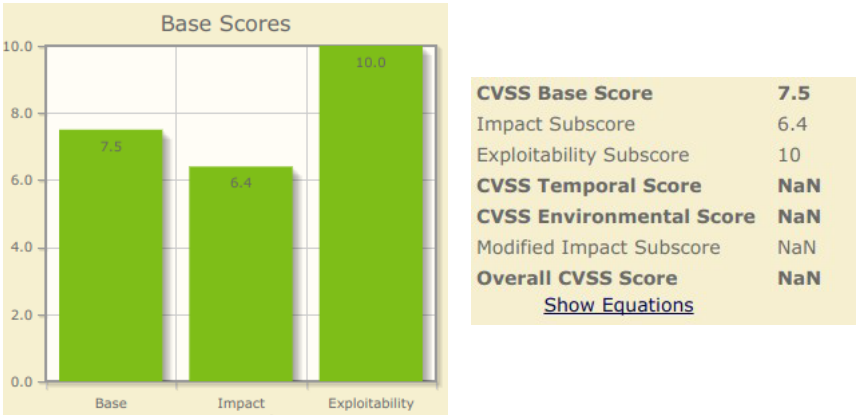
\includegraphics[width=0.6\textwidth]{./Images/cap2/2.21.png}
\end{figure}
\FloatBarrier

Passiamo a considerare le Metriche Temporali:
\begin{itemize}
    \item Sono disponibili script per l’esecuzione dell’exploit,
quindi E:H
    \item E’ stata rilasciata una nuova versione di BASH che
elimina il difetto, quindi RL:OF
    \item La vulnerabilità è vera, quindi RC:C 
\end{itemize}
Otteniamo il punteggio temporale:

\begin{figure}[hbpt!]
    \centering
    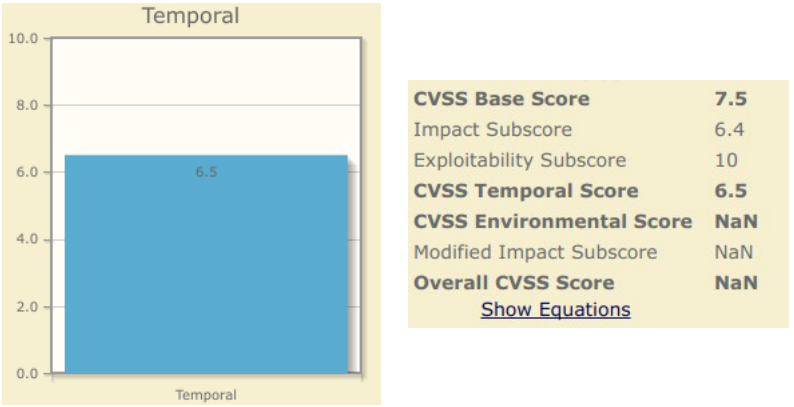
\includegraphics[width=0.6\textwidth]{./Images/cap2/2.22.png}
\end{figure}
\FloatBarrier

Continuiamo con le Metriche Ambientali:
\begin{itemize}
    \item Il danno massimo stimato sul Web server è un
DoS che può rendere molto lento il negozio
    \item Il Web server è l’unico asset soggetto a
CVE-2014-6271, quindi TD:L 
    \item Il Web server esegue con un utente non privilegiato, mentre il database back-end associato al Web server non
memorizza tutte le informazioni aziendali. Pertanto, CR:M, IR:M. AR:M 
\end{itemize}
Otteniamo il punteggio ambientale:

\begin{figure}[hbpt!]
    \centering
    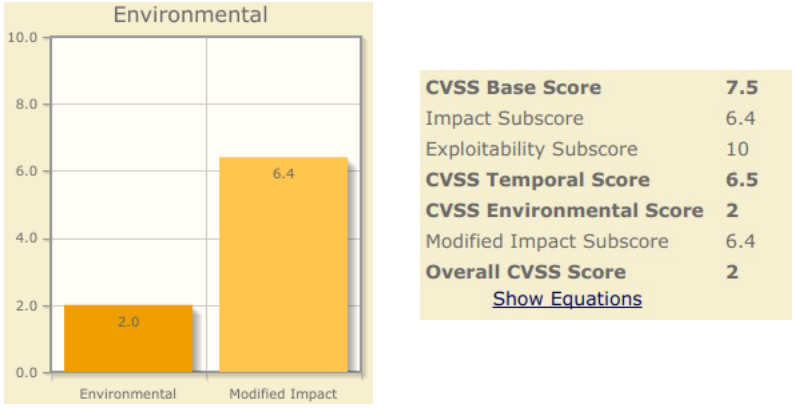
\includegraphics[width=0.6\textwidth]{./Images/cap2/2.23.png}
\end{figure}
\FloatBarrier
Notiamo che, per l’esempio considerato,
il Punteggio Temporale è più basso del
Punteggio Base (esiste infatti una patch ufficiale contro la
vulnerabilità). Inoltre, il Punteggio Ambientale è più basso
del Punteggio Temporale (perché sostanzialmente, si tratta di danni locali).

\let\cleardoublepage\clearpage